% Chapter 1

\chapter{Background} % Main chapter title

\label{Chapter1} % For referencing the chapter elsewhere, use \ref{Chapter1} 

%----------------------------------------------------------------------------------------

\section{Problem definition}

Optimization, the act of finding the best action in a given situation, is both a ubiquitous problem and one of a great importance. Mathematically, the \textit{global} optimization of a real-valued function $f:\D \to \mathbb{R}$ aims to find a minimizer $\x^\star$ (there may be more than one) in the search space $\D$, such that:
%
\begin{equation} \label{eq:1.1}
\x^\star = \argmin_{\x\in\D} f(\x)
\end{equation}
%
Considering $g(\x) = -f(\x)$ shows, as would be expected, that maximization is equivalent. The function $f$ to be optimized is referred to as the \textit{objective function}. In contrast to local optimization, global optimization requires that $f(\x^\star) \leq f(\x)$ for \textit{all} $\x \in \D$ rather than only in some neighbourhood about $\x^\star$. In this project, we assume that the search space $\D$ is a compact subset of  $\mathbb{R}^d$ where $d \in \mathbb{N}$.

This problem, given by equation \ref{eq:1.1}, is the subject of a vast array of scientific literature. In practise, the objective function $f$ may additionally have the following challenging properties P1 - P4:
%
\begin{enumerate}[label={P}{\arabic*}]
\item{ \label{itm:p1}
\textbf{Non-linear, non-convex}: In general, the objective function cannot be assumed to be linear or, more broadly, convex. The extensive fields of linear programming and convex optimization study these cases respectively. \citet{rockafellar1993lagrange} famously describes that in truth the ``great watershed in optimization'' lies between the difficulty of the convex and non-convex cases.
}
\item{ \label{itm:p2}
\textbf{Black-box}: A function is called \textit{black-box} if it can only be viewed in terms of its inputs and outputs. If $f$ is black-box then it does not have analytic form or derivatives, such as the gradient $\nabla f$ or Hessian $\mathbf{H}$, which can be reasoned about and, in particular, used in the search for $\B{x}^*$. As \citet{vizier} note in their paper about Google's in-house black-box optimizer:
%
\begin{quotation}
``Any sufficiently complex system acts as a black-box when it becomes easier to experiment with than to understand''
\end{quotation}
%
To this end, they suggest that as the systems we create, and hope to optimize, increase in complexity, black-box optimization techniques will become increasingly important. For problems with this property, optimization may only proceed by querying $f$ point-wise at inputs $\x\in\D$ in order to learn about its behaviour.
}
\item{ \label{itm:p3}
\textbf{Expensive to evaluate}: The sampling procedure is computationally, economically or otherwise prohibitively expensive. Most prevalently the objective function is time-consuming to evaluate. For example, when tuning the hyper-parameters of a machine-learning model, each function evaluation is potentially very time-intensive as it corresponds to training and evaluating the performance of the primary model \citep{snoek2012practical}. That being said, there are many examples of more general costs. In chemistry, in order to optimize the yield of a reaction, evaluating the objective function involves potentially resource-intensive and laborious experiments. No matter the resource in question, practitioners have finite budgets and, as a result, may only be able to afford relatively few function evaluations. Often it is specified that the number of function evaluations which can be afforded is $N$- which we will take to be the case in this project. More general formulations may, among other considerations, take into account the variable costs of sampling at different locations \cite{snoek2012practical}.
}
\item{ \label{itm:p4}
\textbf{Noisy}: When $f$ is evaluated at $\x$, the value returned $y$ is contaminated by noise $\epsilon$, assumed to be Gaussian with zero mean and variance $\sigma^2$ such that $y = f(\x) + \epsilon$. Problems of this sort are described as \textit{stochastic programming} problems.
}
\end{enumerate}

This project will begin in Chapters \ref{Chapter1}, \ref{Chapter2} and \ref{Chapter3} with an introduction to \textit{Bayesian optimization}, which is a state-of-the-art method intended for optimizing objective functions with the above properties. 

Bayesian optimization and related approaches have a rich history. Their popularity among practitioners and researchers is steadily increasing \cite{shahriari2016taking}. 

\newpage

\section{Pragmatic aims} \label{sec:prag}

Solving equation \ref{eq:1.1}, namely finding a minimizer $\x^\star$, with the additional challenges \ref{itm:p1}-\ref{itm:p3} is a difficult undertaking (leaving \ref{itm:p4} a moment). If it is assumed that $f$ is Lipschitz-continuous, that is
%
\begin{equation}
\nonumber \exists \, l \geq 0 \quad\mathrm{s.t.}\quad \forall \, \x, \x' \in \D, \quad \lvert f(\x) - f(\x') \rvert \leq l \lvert \x - \x' \rvert,
\end{equation}
%
then it can be guaranteed that a minimizer $\x^\star$ exists \citep{horst2013handbook}. However, finding it in general is not possible using a finite number of function evaluations \citep{lizotte}. Even guaranteeing a solution evaluates to within $\epsilon$ of the true maximum $f(\x^\star)$, which we will call \textit{$\epsilon$-optimality}, requires a minimax approach where a grid of samples are made with resolution proportional to $\epsilon$ \citep{betro1991}. Sometime called the ``curse of dimensionality'', the number of points in such a grid scales exponentially with the dimension $d$, which quickly becomes impractical even in low dimensions due to property \ref{itm:p2}. The situation is only made worse if evaluating the objective function is also noisy, \ref{itm:p4}. For this reason, some clarification is required on the aims of optimization in the face of what is considerable adversity. 

\citet{lizotte} proposes a principle of perseverance, noting that although the problem is difficult that doesn't make it go away. The world is full of difficult optimization problems that we would still like to make progress on. The good news is that overwhelmingly the task is not all-or-nothing. That is, suboptimal solutions may be perfectly viable if the contextual performance difference is small. In some situations, perhaps when sampling has a meaningful financial cost for example, a cheap suboptimal solution may even be preferred. Furthermore, the previous minimax approach pays a high price to insure against worst-case, pathological scenarios which may not be very plausible in reality \citep{brochu2010interactive}. 

These considerations motivate a ``practical'' \citep{lizotte} or ``average-case'' \citep{streltsov1999non} approach, where the focus is in finding a ``good'' solution or converging on a minimizer $\x^\star$ in few evaluations, rather than in making theoretical guarantees about optimality. This is the philosophy that we will adopt during this project.

\section{Sample designs} \label{sampledesigns}

How, then, should points be queried to efficiently learn about $\x^\star$ so that the above aims can be met?

We first present two relatively naive strategies: \textit{grid-search} and \textit{random-search}. These approaches directly select a set of points, called a sample design, to be evaluated. Grid-search is previously mentioned above, where a dense grid was used by \citet{betro1991} to ensure $\epsilon$-optimality. Of course, the resolution need not be so high. More generally, in a grid-search samples are taken spaced evenly throughout the domain $\D$ at a resolution appropriate to the optimization budget. Although the whole domain is superficially covered, if few function evaluations can be afforded then this coverage is too sparse to reliably locate a minimizer. Meanwhile, random-search simply chooses inputs in the domain $\D$ to evaluate at random.

Perhaps counter-intuitively, \citet{bergstra2012random} show that in some sense random-search actually performs more efficiently than grid-search. In particular, grid-search performs very poorly when the objective function $f$ has a low effective dimensionality. This is because multiple sample points have the same value when collapsed down onto any dimension. Looking at it another way, if one of the dimensions has little impact then in a grid-search many samples are entirely wasted - without learning \textit{anything} about the other dimensions. That being said, random-search is also severely flawed: complete randomness lends itself to clumps of points and large areas left empty. 

One way of overcoming these problems is to use a space-filling, but still random, design such as the \textit{latin-hypercube} \cite{lectures}. Latin-hypercube designs generalize the latin-square, which is a grid with exactly one sample in each column and each row, to arbitrary dimension. This avoids the problem of collapsing, from which grid-search suffers. Figure \ref{fig:1i} gives an example of the usage of each of grid-search, random-search and latin-hypercube sampling on a two dimensional objective function. 

\begin{figure}
\centering
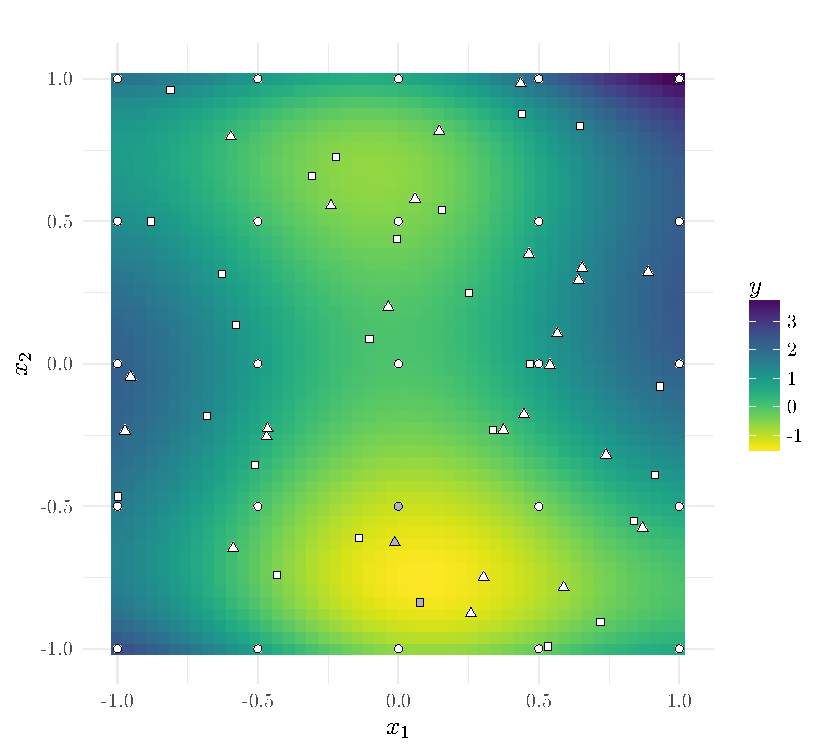
\includegraphics[scale=1]{fig1i.pdf}
\begin{tabular}{ l | l c c }
              & Symbol & $y_{\mathrm{min}}$ & $(x_1, x_2$)\\ \hline
  Grid-search & Circles & -1.050 & $(0.000, -0.500)$\\
  Random-search & Triangles & -1.322 & $(0.131, -0.638)$\\
  Latin-hypercube & Squares & -1.382 & $(0.078 -0.837)$\\
\end{tabular}
\caption[width=\linewidth]{Density plot of modified two-dimensional camel function $y = (4 - 2.1x_1^2 + 0.3x_1^4)x_1^2 + (x_1+0.6)x_2 + (-4+4x_2^2)x_2^2$ on the square $x_1 \in [-1,1], x_2 \in [-1,1]$. 25 points sampled from each of grid-search, random-search and latin-hypercube sampling; minimum found by each method shown in grey. True global minimum is -1.470 at $(0.094, -0.747)$.} \label{fig:1i} 
\end{figure}

\section{Models \& trade-offs}

Although there are many more complicated and arguably better sample designs than the ones described above, it is intuitively clear that any such strategy is suboptimal: information gained during the search is not used to better inform the next decision. Rather than choose all the points at once it makes sense instead to consider a sequential decision making problem where at each stage a point is carefully chosen to be evaluated next. The same philosophy is true of many situations. It would be unwise to require students starting at Durham to choose their modules for first, second and third year all at once as their preferences will surely change as they learn more.

So, how can this information be used? It is important to note that in order to learn about the behaviour of the objective function where it has not been specifically sampled we must make some assumptions about how the data we have may be extrapolated. In particular, we assume that points close in input are to some extent close in output. In other words, that $f$ is somewhat smooth. Making assumptions, like this one, about the nature of the objective function is helpful if those assumptions are right. If they are not too strong or restrictive, then \textit{on-average} they will be right \cite{blog}. This is the foundational idea of the model-based approach to optimization, in which statistical inference can be used to aid in the search process.

Assuming that the objective function $f$ is smooth, there are two types of location which should be the focus of the search. Firstly, sampling in uncertain regions, not near to any previous evaluations, will provide helpful information about the global behaviour of the objective function. On the other hand, sampling in promising regions, near to previous low evaluations, will allow solutions to be refined locally. We will term these two contrasting ideas as \textit{global search} and \textit{local search}, respectively. This is slightly non-standard terminology, the reason for which will be explained shortly in section \ref{sec:bandits}.

Good strategies then must appropriately balance global search and local search. Too great a focus on global search leads to the optimization never converging on a solution. Conversely, too great a focus on local search tends to locate local rather than global minimizers.

The sample designs given in section \ref{sampledesigns} are all examples of strategies which neglect local search. Once they find a promising location they would be better served to invest more of their attention in that area - so that they may informally ``drill-down'' \cite{lectures} to a better solution.

On the other hand, for example techniques which iteratively alter solutions in order to get an idea of the gradient, with the idea being to move in the direction of greatest decrease, have too great a focus on local-search. A ball on the surface of figure \ref{fig:1i} will roll into the local minima (rather than the global minima) if is placed too close - in the so-called \textit{basin of attraction}. In practise this problem may be remedied by random restarts, i.e. repeating the search a number of times with the ball placed randomly each time. However, this alteration is not viable in view of property \ref{itm:p4}. The fact that the local minima is a global minima when the objective function is convex is what makes convex optimization significantly more approachable than the general case.

\newpage

\section{Bayesian optimization} \label{BO}

Bayesian optimization \citep{kushner1964new} \citep{mockus1974bayesian} aims at addressing the optimization of objective functions with the above properties \ref{itm:p1}-\ref{itm:p3} and possibly \ref{itm:p4}. It is a sequential, model-based optimization algorithm which learns from all available observations to make better informed choices about the next point to query. The algorithm is detailed in algorithm \ref{algo:1} and has two key components: the statistical \textit{emulator} and the \emph{acquisition function}. 

As $f$ is black-box, there is uncertainty about its true value where it has not been directly evaluated (and when $f$ is noisy then even at evaluated points as well). It is theoretically justified \citep{cox} that Bayesian probability theory is a rational way to reason about such uncertain states of knowledge. Prior beliefs about the objective function and data-generation mechanism may be encapsulated with an explicit, probabilistic, statistical model. 

\begin{figure}
\begin{flushleft} \hspace{25pt} (a) Stage $n=1$ \end{flushleft}
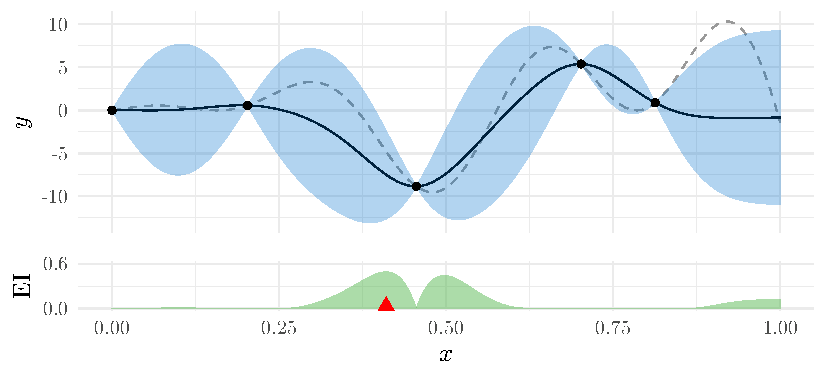
\includegraphics[scale=1]{fig1iia.pdf}
\begin{flushleft} \hspace{25pt} (b) Stage $n=2$ \end{flushleft}
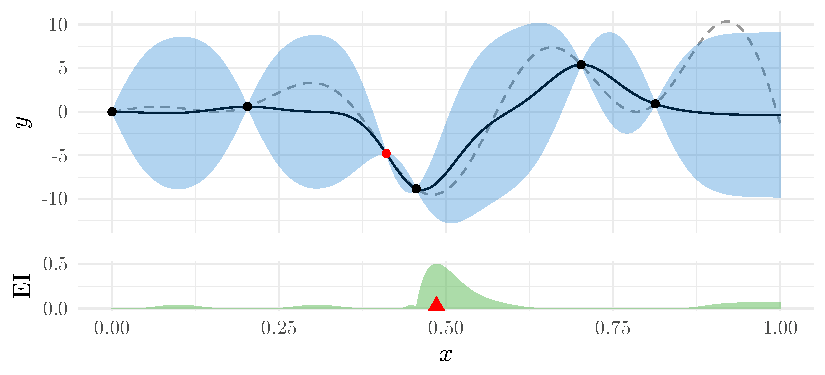
\includegraphics[scale=1]{fig1iib.pdf}
\centering
\caption{A two-stage example run of Bayesian optimization. Objective function $f(x) = 10x(\sin(10x) + \cos(20x))$ is shown as the dahsed grey line in both (a) and (b). The mean of the Gaussian process emulator, i.e. the surrogate function, at each stage is shown as the solid black line. Uncertainty about the objective function is shown as the light-blue point-wise $95\%$ confidence region. The initial data-set $\Da_0$ is five points and their noise-free evaluations generated by latin hyper-cube sampling. The acquisition function is shown in green, with its maximum at each stage shown by the red arrow. Here we use the one particular acquisition function, expected improvement (EI), which will be properly introduced in Chapter \ref{Chapter3}. The acquisition function maximum in (a) is shown evaluated as the red circle in (b).} \label{fig:1ii}
\end{figure}

This probabilistic model is known as an emulator \cite{lectures}. It should behave similarly to the objective function $f$, but be much cheaper to work with. The emulator provides a predictive distribution for $f$ evaluated at new inputs. The mean of this distribution may be used as a \textit{surrogate} for the objective function and the variance allows for uncertainty quantification.  When data $\{\x, y\}$ is observed then the model can be sequentially updated and refined, using Bayes' rule. 

Typically the emulator used is a \textit{Gaussian process}, which is a convenient and flexible model for this purpose. We will introduce Gaussian processes and their role in Bayesian optimization in more detail in Chapter \ref{Chapter2}.  

To guide the search for a global minimizer, the emulator is leveraged by an acquisition function, sometimes also called an in-fill function. It is a function of the state of the optimization at the current stage $n$, i.e. all of the data which is available and the Gaussian process emulator to the objective function $f$, which returns a suggestion of the next point to sample $\x_n$. This function automatically balances the trade-off between global and local search. Many possible acquisition functions have been proposed in the literature. This will be explored in more depth in Chapter \ref{Chapter3}. 

% Algorithm: General Bayesian Global Optimization 
\begin{algorithm}
\SetAlgoLined
\textbf{input} objective function $f$, acquisition function $\alpha$, initial dataset $\Da_0$\;
 \For{$n = 1, 2, \ldots, N$}{
  Fit Gaussian process to dataset at stage $n$, $\Da_{n-1}$\;
  Maximize acquisition function $\alpha$ over Gaussian process to propose next point to sample, $\x_{n}$\;
  Query objective function $f$ at $\x_{n}$, returning $y_{n} = f(\x_{n}) + \epsilon$\;
  Augment dataset $\Da_{n} = \Da_{n-1} \cup \{\x_{n}, y_{n}\}$\;
 }
Fit Gaussian process to complete dataset $\Da_{N}$\;
\Return{\textrm{recommendation} $\x^-$}\;
\vspace{5pt}
\caption{Bayesian optimization algorithm} \label{algo:1}
\end{algorithm}

Figure \ref{fig:1ii} gives a toy example of the use of Bayesian optimization for a one-dimensional objective function, illustrating stages $n=1,2$ in algorithm \ref{algo:1}. In this example, the optimization begins with an already available data-set $\Da_0$ which is used to build the inital Gaussian process emulator. It has been suggested that in general a small number of points, depending on the dimension, should be sampled prior to the start of sequential optimization \cite{bischl2017mlrmbo}. After the budget has been spent, the algorithm returns a \textit{recommendation} $\x^-$ which it is hoped is a global minimizer. The recommendation is typically the best performing $\x_n$ or the minimizer of the final surrogate function.

One thing that should be clarified is that when the properties stated, particularly \ref{itm:p3}, are \textit{not} the case then it is more than likely that another algorithm will perform better than Bayesian optimization. It is a topic of recent research extending Bayesian optimization to make use of additional information, such as gradients \cite{lizotte}, if it is available. 

\section{Bandits} \label{sec:bandits}

A similar premise to the problem we have been considering is the so-called \textit{multi-armed bandit} problem \citep{robbins1985some}. Imagine that a gambler has just one night at a casino and a number of slot-machines (also known as bandits) which can be played. At each stage the gambler must choose an arm to play, with each arm having different odds of paying out. How should the gambler select arms to play in order to maximize their return over the night?

To provide a broader context for Bayesian optimization, we briefly discuss some of the differences between the two problems.

As rewards can be collected at each stage, the multi-armed bandit problem is what is known as an online learning problem \citep{ryzhov2012knowledge}. In the Bayesian optimization setting we are typically only concerned with the performance of the final recommendation of the algorithm $\x^-$, which is contrast is referred to as offline learning. That being said, there is some recent research into online Bayesian optimization, for instance the optimization of financial portfolios \cite{nyikosa2015adaptive}.

The distinction between on and offline learning is similar to that between summative and formative assessed work. In online learning problems the agent must trade-off between explorative behaviour which sacrifices immediate rewards in the hope of longer-term gains and exploitative, myopic behaviour which greedily aims to do the best it can at the present iteration \citep{gelbart}. For example, in the multi-armed bandit problem choosing to play a new unknown, possibly poor, arm is explorative behaviour, whereas playing the arm with the best odds found so far is exploitative behaviour. Many authors use the terminology exploration and exploitation to refer to the what we have termed called global and local search.

Another difference is that the bandit setting is discrete, whereas we consider the domain $\D$ to be continuous. In addition, it is not assumed that the arms have spatial interpretation, i.e. that the behaviour of a given arm can be inferred from that of adjacent arms, whereas we assume that function evaluations are informative for nearby locations.

Finally, the bandit literature often places a greater emphasis on long-run convergence rates and theory than Bayesian optimization \cite{gelbart} which, as we discuss in section \ref{sec:prag}, often can't afford to make such guarantees and is more pragmatic as a result.



